\section{Particle Tracking}

The CLAS12\cite{Burkert:2020akg} detector is built around a six-coil toroidal magnet which divides the active detection into six azimuthal regions, called "sectors". Each sector is equipped with three regions of drift chambers. Each region consists of two chambers (caller super-layers), with each of them having 6 layers of wires. Each layer of wires in super-layer contains 112 wires making a super-layer a 6x112 wire matrix. The schematic view of one super-layer is shown on Figure~\ref{dc:side_view} (right panel).

\begin{figure}[!ht]
\begin{center}
 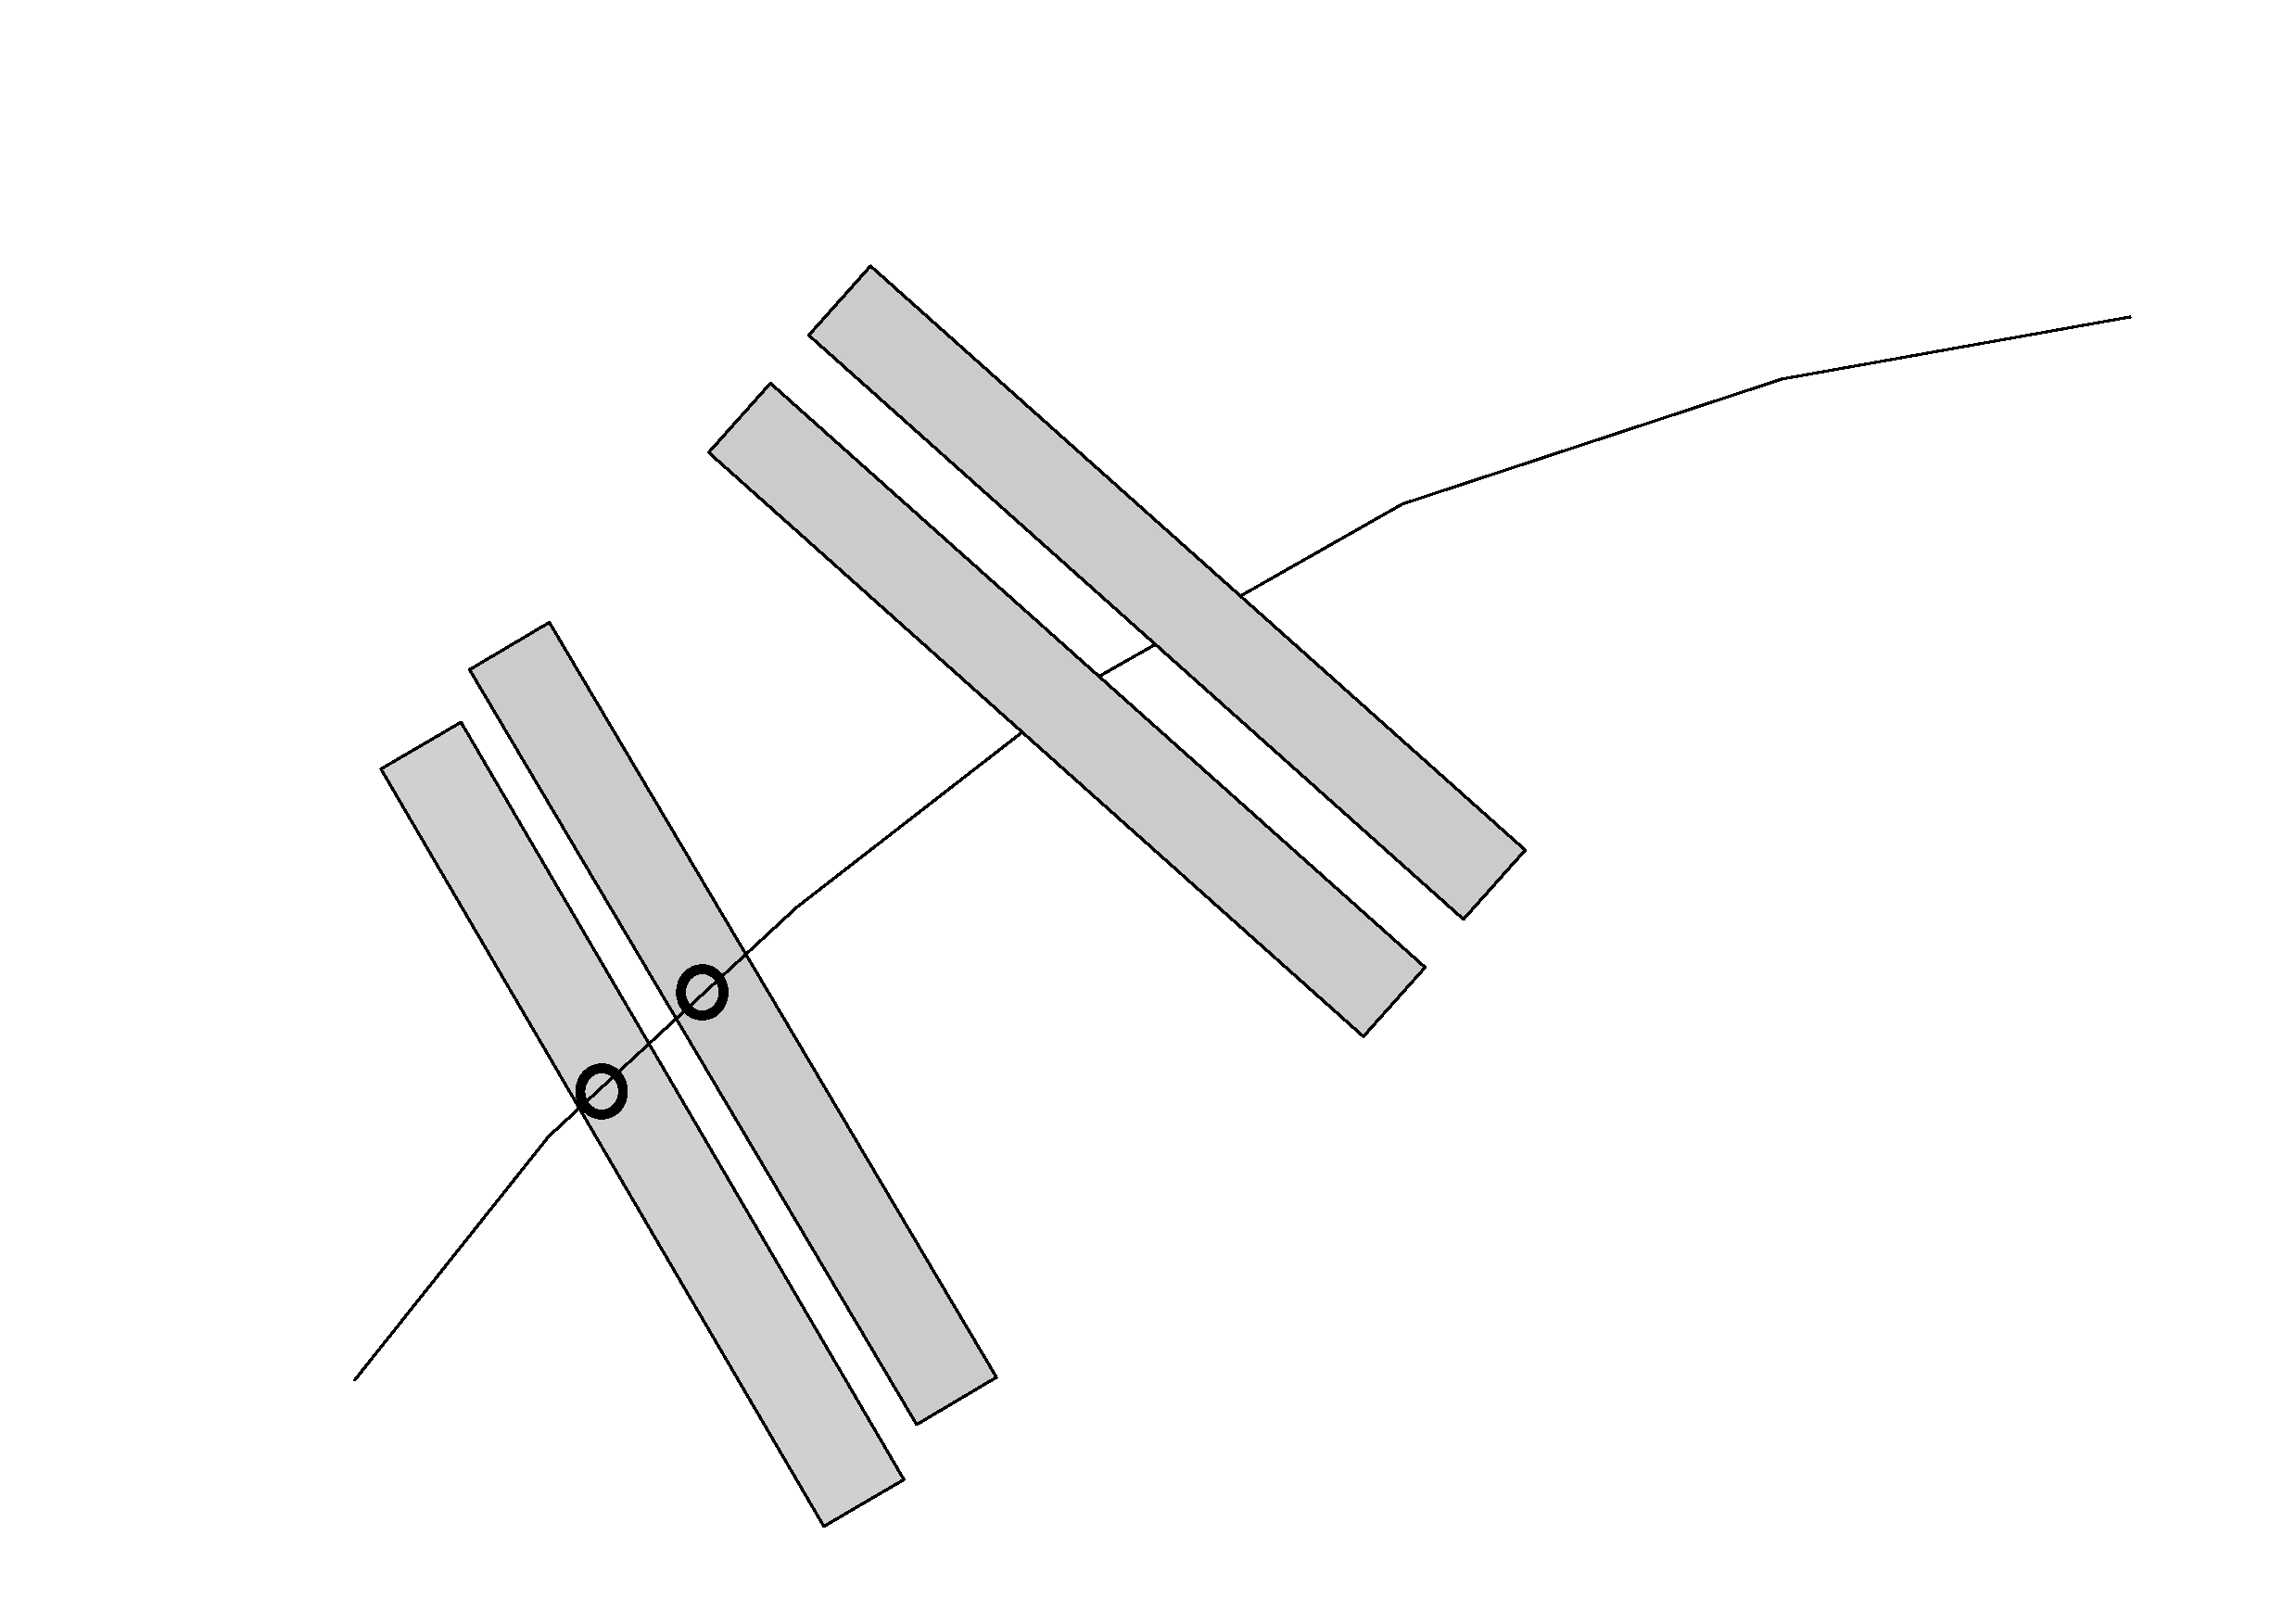
\includegraphics[width=3.5in]{images/dc_side_view.pdf}
 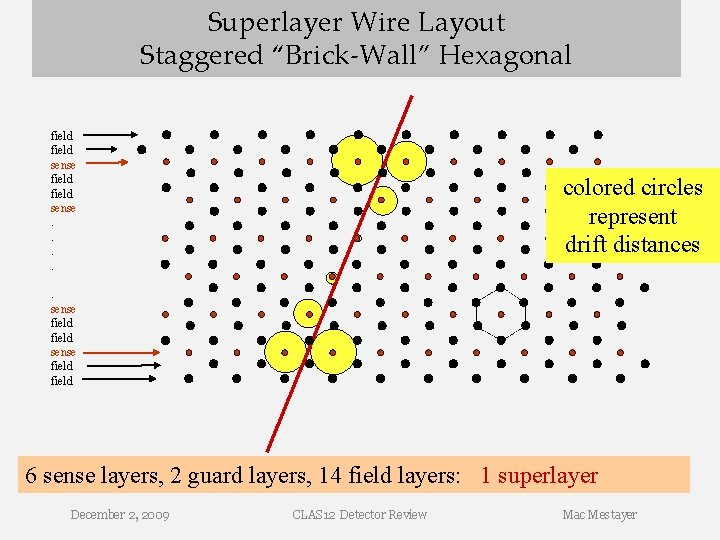
\includegraphics[width=2.5in]{images/image-29.jpg}
\caption {Side and front view of drift chambers. a) the layout for one sector showing three regions of drift chamber. Z-axis is direction of incoming beam. b) diagram of wire directions in each super layer.}
 \label{dc:side_view}
 \end{center}
\end{figure}

Particle that originates at interaction vertex in forward direction that pass through all three regions of the drift chamber in given sector are reconstructed by tracking algorithms. First adjacent  wires in each super-layer with a signal are grouped together into clusters (called segments), then track candidates are constructed by forming 6 segment combinations (one per each super-layer). Each track candidate is validated by tracking algorithm by performing a polynomial fit to determine if the candidate can be a real track. Once track candidates are isolated they are further refined using Kalman filter to measure particle parameters (such as momentum and angles). 
There are many experiments conducted with CLAS12 detector which have different running conditions (i.e. different targets and beam currents).
The changing beam energies and beam intensities (current) affect the amount of background that is detected in each detector components. For drift chambers the added background can be in a form of random hits that can be isolated by noise reducing algorithm, and can be in form of segments that do not belong to a track. With increased luminosity (beam current and target combination) number of combinatorics and the candidates to consider significantly increases, and this leads to decreased efficiency in track reconstruction. Recent studies done with experimental data and simulation showed that the tracking efficiency decreases with a rate of $0.44\%$ per nA of beam current. This leads to tracking efficiency at standard experimental running conditions (which is $45~nA$ electron beam incident on $40~cm$ liquid hydrogen target) is $\approx 80\%$.
The decrease of the efficiency of tracking what prevents experiments to run at higher beam currents (interaction rates), and increasing tracking efficiency will allow experiments to run for shorter time to collect desired statistics for physics results. 